\documentclass[11pt]{amsart}
\usepackage[centering]{geometry}           % See geometry.pdf to learn the layout options. There are lots.
\geometry{a4paper} % ... or a4paper or a5paper  or ... letterpaper
%\geometry{landscape}                % Activate for for rotated page geometry
%\usepackage[parfill]{parskip}    % Activate to begin paragraphs with an empty line rather than an
%indent
\usepackage{graphicx}
\usepackage{amssymb}
\usepackage{epstopdf}
\usepackage{amsmath}
\usepackage{subcaption}
\usepackage{wrapfig}
\usepackage{lscape}
\usepackage{rotating}
\setlength{\rotFPtop}{0pt plus 1fil}% <- add this line after loading rotating
\setlength{\rotFPbot}{0pt plus 1fil}% <- maybe its better to add this line too
\DeclareGraphicsRule{.tif}{png}{.png}{`convert #1 `dirname #1`/`basename #1 .tif`.png}






\title{Stellar Oscillations Tidally Induced by a Planetary Companion}
\author{Andrew Bunting}
%\date{}                                           % Activate to display a given date or no date
%
\begin{document}

\maketitle



\section{Introduction} \label{Introduction}

This explains the maths (and hints at its implementation) used to convert the outputs of my stellar oscillation code into either a lightcurve or a spectrum for the photometric and RV detection of tidally induced oscillations respectively.



\subsection{Starting point} \label{Intro:StartingPoint}

The inputs required to do these calculations include the properties of the star, both in equilibrium and perturbed: $R$, the stellar equilibrium radius; $F_{0}$, the equilibrium surface flux; $\vec{\xi}$, the vector displacement of the surface; and $\vec{F}'$, the vector perturbation to the flux at the surface (although this is the Eulerian perturbation, and we will need to use the Lagrangian perturbation, which is a simple conversion of $\Delta \vec{F} = \vec{F'} + ( \vec{\xi} \cdot \vec{\nabla} ) \vec{F}_{0}$ ).  Properties of the driving mechanism for the oscillation mode are also needed: $\omega$, the frequency of the orbit; $l$ and $m$, the degree and order of the spherical harmonic of the oscillation mode; and $\Phi =  f R^{2}$, the perturbing potential at the surface.

The coordinate system to be used must also be defined.  We will be using spherical coordinates based upon the star-planet system, with the direction to the planet at $(\theta, \phi) = (\frac{\pi}{2}, 0)$ at $t = 0$, and evolving as $(\frac{\pi}{2}, \omega t)$.  Therefore, the poles of the coordinate system (that is, where $\theta = 0 \, \text{or} \, \pi$) are perpendicular to the plane of the planet's orbit.  The direction to the observer is defined within these coordinates as $(\theta_{o}, \phi_{o})$, defining $\hat{n}_{o}$ as the unit vector pointing in this direction.





\section{Radial Velocity} \label{RV}

The motion of the surface induced by the tidal perturbation results in a spectroscopic change, due to the Doppler effect - a broadening of linewidth, and potentially a shift in the line's central frequency.

\subsection{Mathematical overview} \label{RV_overview}

The core of this depends upon keeping track of the vector motion of the surface, using:

\begin{equation}
\vec{v} = \frac{\partial}{\partial t} \vec{r} = \frac{\partial}{\partial t} ( R \hat{r} + \vec{\xi} ) = \frac{\partial}{\partial t} \vec{\xi} .
\end{equation}

The radial velocity measured is the projection of this surface velocity along the line of sight of the observer:

\begin{equation}
v_{RV} = \vec{v} \cdot \hat{n}_{o}.
\end{equation}

To calculate the effect on an idealised emission line, both the radial velocity and the luminosity of the surface element must be known.  The perturbation to the luminosity of the surface element due to the tidally induced oscillations is neglected, but the change in luminosity due to the angle between the surface normal and the observer must be taken into account, both in terms of projecting the flux and area to get the luminosity, and in terms of limb darkening.

Limb darkening is given as:

\begin{equation}
h = c \, ( 1 - u (1 - \hat{r} \! \cdot \! \hat{n}_{o}) )
\end{equation}

where the value of $u$ determines the model of limb-darkening that you are using, and $c$ normalises $h$, so that $\int_{0}^{1} \, h \, \mu \, \text{d}\mu = 1$, and therefore $\int h \, \hat{n}_{o} \! \cdot \! \vec{\text{d} S} = \pi$, preserving the total projected area.  For Eddington limb-darkening $c = 1$ and $u = 0.6$.

The luminosity of the surface element requires both the flux and the area to be projected along the line of sight, as shown in figure \ref{fig:flux_diagram}.  This gives us the equation for the luminosity of a surface element as:

\begin{equation}
\text{d}L = h \, \bar{F}_{0} \, \vec{\text{d}S} \! \cdot \! \hat{n}_{o}
\end{equation}

where the equilibrium surface flux, equilibrium surface normal and equilibrium surface element area are all used because the impact on the luminosity of the element will be negligible.

\begin{figure}
\begin{center}
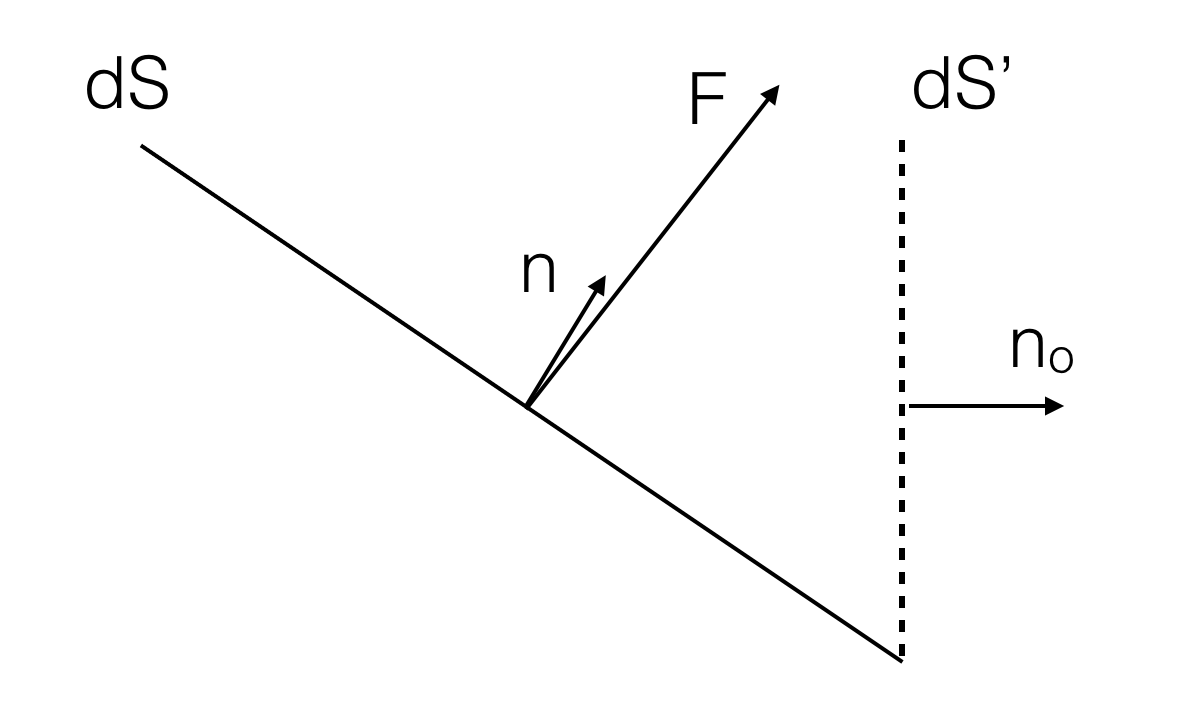
\includegraphics[width = 0.75 \textwidth]{flux_diagram.png}
\caption{This diagram shows the normal to the surface, n; the unit vector towards the observer, $n_{o}$; the surface element of the star, d$S$; the projected surface element, d$S'$; and the vector flux, $F$, which need not be parallel to the surface normal.  Hats and arrows have not been included to denote vectors in the diagram because it was drawn up fairly speedily.  The luminosity from the surface is given by $\vec{F} \! \cdot \! \vec{\text{d}S'}$, which is the power passing through the surface.  The surface then radiates equally in all directions, so the angle-averaged flux should be thought of as a measure of luminosity per unit area, and is therefore a scalar and not a vector, which is $\bar{F} \propto \vec{F} \! \cdot \! \vec{\text{d}S}$.  Therefore the luminosity observed will be equal to this angle-averaged flux multiplied by the projected area of the surface element, $\text{d}S'$; leading to $\text{d}L = \bar{F} \, \hat{n} \! \cdot \! \hat{n}_{o} \, \text{d}S$.}
\label{fig:flux_diagram}
\end{center}
\end{figure}

To combine these to produce the spectrum, the contribution to the luminosity at that radial velocity from each surface element must be summed.  This leads to the summation for each radial velocity bin, $v_{RV_{i}}$:

\begin{equation}
L_{i} = \sum \text{d}L
\end{equation}

where the sum runs over the elements for which both $\hat{r} \cdot \hat{n}_{o} > 0$ and $| v_{RV} - v_{RV_{i}} | < \frac{\delta v_{RV}}{2}$ (where $v_{RV_{i}}$ is the central radial velocity of the bin, and $\delta v_{RV}$ is the bin width) which ensures both that the element is visible and has the appropriate radial velocity for that bin.



\subsection{Implementation} \label{RV:Implementation}

Here I run through a more detailed version of what's going on, including the practicalities of what exactly can be taken directly from the oscillation code, and what you need to do a little calculating to get to.

\subsubsection{Surface velocity} \label{RV:Implementation:SurfVel}

In the $l=2$, $m=2$ spherical oscillation mode, the variables oscillate as:

\begin{equation}
q = \Re \left(  \left( q_{r} + i q_{i} \right)  3 \sin^{2}(\theta) e^{2 i ( \omega t - \phi)}   \right)   =    3 \sin^{2}(\theta) \left(  q_{r} \cos \left( 2 ( \omega t - \phi) \right)  - q_{i} \sin \left( 2 ( \omega t - \phi) \right) \right) 
\end{equation}

which enables $\xi_{r}$, that is, the radial displacement (unfortunately the notation regarding real and radial is a bit confusing, but is usually understood within context), to be calculated easily by substituting it for $q$, the dummy variable in the above equation.  The tangential displacement, however, is not directly calculated by the oscillation code, and therefore requires a bit more work.

Using

\begin{equation} \label{eq:mom_lin}
\rho_{0} \frac{\partial^{2} \vec{\xi}}{\partial t^{2}} = - \vec{\nabla} p' - \rho_{0} \vec{\nabla} \Phi_{P}
- \rho' \vec{\nabla} \Phi_{0}
\end{equation}

the tangential displacement is found to be

\begin{equation}
\vec{\xi}_{\perp} = \Re \left(   \frac{1}{m^{2} \omega^{2}}  \vec{\nabla}_{\perp}  \left(   \frac{p'}{\rho_{0}}  +  \Phi_{p}   \right) \right).
\end{equation}

which, when expressed using the explicit form of the oscillations, becomes

\begin{equation}
\vec{\xi}_{\perp} = \Re \left(   \frac{1}{m^{2} \omega^{2}}  \left(   \frac{p'_{r}}{\rho_{0}}  +  f r^{2} + i \frac{p'_{i}}{\rho_{0}}   \right)   \vec{\nabla}_{\perp}  \left(   3 \sin^{2}(\theta) e^{2 i ( \omega t - \phi)}   \right)  \right)
\end{equation}

where $f = - \frac{G m_{p}}{4 D^{3}}$ is used to replace $\phi_{p}$ according to $\phi_{p} = f r^{2}$

The tangential gradient is given by $\vec{\nabla}_{\perp} = \hat{\theta} \frac{1}{r} \frac{\partial}{\partial \theta} + \hat{\phi} \frac{\partial}{\partial \phi}$.  Using this, and taking the real part gives the final expression for the tangential displacement of the surface:

\begin{multline}
\vec{\xi}_{\perp} =    \frac{6 \sin(\theta)}{r m^{2} \omega^{2}}  \Bigg\{  \left(   \frac{p'_{r}}{\rho_{0}}  +  f r^{2} \right) \left[ \cos(2( \omega t - \phi )) \cos(\theta) \hat{\theta}  +  \sin(2( \omega t - \phi )) \hat{\phi} \right] \\
 + \frac{p'_{i}}{\rho_{0}}  \left[ \cos(2( \omega t - \phi )) \hat{\phi}  -  \sin(2( \omega t - \phi )) \cos(\theta) \hat{\theta} \right]    \Bigg\}.
\end{multline}

By recalling the full form of the radial displacement, we have the full vector form of the displacement:

\begin{multline}
\vec{\xi} =    3 \sin^{2}(\theta) \left(  \xi_{r} \cos \left( 2 ( \omega t - \phi) \right)  - \xi_{i} \sin \left( 2 ( \omega t - \phi) \right) \right) \hat{r} \\
+ \frac{6 \sin(\theta)}{r m^{2} \omega^{2}}  \Bigg\{  \left(   \frac{p'_{r}}{\rho_{0}}  +  f r^{2} \right) \left[ \cos(2( \omega t - \phi )) \cos(\theta) \hat{\theta}  +  \sin(2( \omega t - \phi )) \hat{\phi} \right] \\
 + \frac{p'_{i}}{\rho_{0}}  \left[ \cos(2( \omega t - \phi )) \hat{\phi}  -  \sin(2( \omega t - \phi )) \cos(\theta) \hat{\theta} \right]    \Bigg\}.
\end{multline}

which is converted into the surface velocity by taking the partial time derivative, giving, when grouped according to unit vector:

\begin{multline} \label{eq:vprime_full}
\vec{v'} = \frac{\partial \vec{\xi}}{\partial t} =    - 6 \omega \sin^{2}(\theta) \Big(  \xi_{r} \sin \left( 2 ( \omega t - \phi) \right)  + \xi_{i} \cos \left( 2 ( \omega t - \phi) \right) \Big) \hat{r} \\
+ \frac{12 \sin(\theta)}{r m^{2} \omega}  \Bigg\{  - \left[ \left(   \frac{p'_{r}}{\rho_{0}}  +  f r^{2} \right) \sin(2( \omega t - \phi ))  + \frac{p'_{i}}{\rho_{0}} \cos (2( \omega t - \phi )) \right]  \cos(\theta) \hat{\theta}  \\
+  \left[ \left(   \frac{p'_{r}}{\rho_{0}}  +  f r^{2} \right) \cos (2( \omega t - \phi )) - \frac{p'_{i}}{\rho_{0}} \sin(2( \omega t - \phi )) \right] \hat{\phi}    \Bigg\}.
\end{multline}


\subsubsection{Radial Velocity} \label{RV:Implementation:RV}

For simplicity, equation \ref{eq:vprime_full} will be rewritten as:

\begin{equation} \label{eq:vprime_short}
\vec{v'} = v'_{r} \hat{r} + v'_{\theta} \hat{\theta} + v'_{\phi} \hat{\phi}
\end{equation}

where the components can be found by comparing equation \ref{eq:vprime_short} with equation \ref{eq:vprime_full}.

To get the measured radial velocity, the surface velocity must be projected along the line of sight of the observer, giving

\begin{equation}
v_{RV} = \vec{v'} \cdot \hat{n}_{o}.
\end{equation}

This is most simply done using the cartesian coordinate system with $\hat{x}$ aligned with the vector pointing to the planet at $t = 0$, $\hat{y}$ pointing to the planet at $\omega t = \frac{\pi}{2}$, and $\hat{z}$ aligned with the angular momentum vector of the system.  In these coordinates, we have:

\begin{equation}
\hat{n}_{o} = \sin(\theta_{o}) \cos(\phi_{o}) \hat{x} + \sin(\theta_{o}) \sin(\phi_{o}) \hat{y} + \cos(\theta_{o}) \hat{z}
\end{equation}

\begin{equation}
\hat{r} = \sin(\theta) \cos(\phi) \hat{x} + \sin(\theta) \sin(\phi) \hat{y} + \cos(\theta) \hat{z}
\end{equation}

\begin{equation}
\hat{\theta} = \cos(\theta) \cos(\phi) \hat{x} + \cos(\theta) \sin(\phi) \hat{y} - \sin(\theta) \hat{z}
\end{equation}

\begin{equation}
\hat{\phi} = - \sin(\phi) \hat{x} + \cos(\phi) \hat{y}
\end{equation}


\subsubsection{Converting this to code}  \label{RV:Implementation:Code}

I will briefly describe how this maths is actually implemented in the code, which is largely a brute force approach.

For each point in time over the course of a planetary orbit, a spectrum must be calculated.  Therefore $\omega t$ is quantised and runs from $0$ to $\pi$ (as the oscillations have twice the frequency of the planetary orbit).

At each value of $\omega t$, every surface element of the star will be assessed and will only have its luminosity included if $\hat{r} \! \cdot \! \hat{n}_{o} > 0$, such that that surface element is visible at that point in time.  For each visible surface element, the luminosity and radial velocity will both be calculated.  The radial velocity determines which bin to add the luminosity, and once the sum has run over the whole star, the spectrum for that timestep is complete, so it is therefore saved.  Then the luminosities can be reset and the process starts again for the next timestep.








\section{Luminosity variation} \label{Lum}

In this section, the method for producing the lightcurves due to the oscillations is covered.  To do this, the first order change in each variable in the integral must be computed.  Each variable will have its own subsection.

The full integral, just as a refresher, is:

\begin{equation}
L = \int \int h \, \bar{F} \, \hat{n}_{o} \! \cdot \! \hat{n} \, \text{d}S
\end{equation}

where $\bar{F}$ is the angle-averaged flux, which can be re-expressed as:

\begin{equation}
L + \Delta L = L + \Delta L_{h} + \Delta L_{F} + \Delta L_{n} + \Delta L_{S}
\end{equation}

where $\Delta L_{h}$ is the change in luminosity due to the effect of the perturbation on limb-darkening, $\Delta L_{F}$ is the change in luminosity due to the perturbed flux, $\Delta L_{n}$ is the change in luminosity due to the change in surface normal, and $\Delta L_{S}$ is the change in luminosity due to the change in surface area.

\subsection{Change in Limb-darkening} \label{Lum:LD}

We start with the general limb-darkening formula:

\begin{equation}
h = c \, ( 1 - u (1 - \hat{n} \! \cdot \! \hat{n}_{o}) )
\end{equation}

which is obviously perturbed by the change in surface normal, to give:

\begin{equation}
\Delta h = c \, \Delta \hat{n} \! \cdot \! \hat{n}_{o}
\end{equation}

which leads to

\begin{equation}
\Delta L_{h} = \int \int \Delta h \, \bar{F} \, \hat{n}_{o} \! \cdot \! \hat{n} \, \text{d}S
\end{equation}



\subsection{Change in flux} \label{Lum:F}

For this, the perturbation to the angle-averaged flux replaces the equilibrium flux to give

\begin{equation}
\Delta L_{F} = \int \int h \, \Delta \bar{F} \, \hat{n}_{o} \! \cdot \! \hat{n} \, \text{d}S
\end{equation}

where $\Delta \bar{F}$ is the perturbation to the angle-averaged flux.  This comes from

\begin{equation}
\bar{F} \propto \frac{1}{2} \vec{F} \! \cdot \! \vec{\text{d}S} = \frac{1}{2} \vec{F} \! \cdot \! \hat{n} \, \text{d}S
\end{equation}

which becomes, to first order

\begin{equation}
\bar{F} \propto \frac{1}{2} \vec{F}_{0} \! \cdot \! \hat{r} \, \text{d}S  +  \frac{1}{2} \vec{F'} \! \cdot \! \hat{r} \, \text{d}S  +  \frac{1}{2} \vec{F}_{0} \! \cdot \! \Delta \hat{n} \, \text{d}S
\end{equation}



\subsection{Surface Normal} \label{Lum:Norm}

To find the normal to the surface, we normalise $\frac{\partial \vec{r}}{\partial \theta} \times \frac{\partial \vec{r}}{\partial \phi}$ where $\vec{r}$ defines the surface of the star as a function of $\theta$ and $\phi$.

This leads to:

\begin{equation}
\hat{n} = \hat{r} + \Delta \hat{n}
\end{equation}

where no re-normalisation is required because the normalisation constant is, to first order, $1$.  This is found to be

\begin{equation}
\hat{n} = \hat{r} - \frac{1}{R} \frac{\partial r}{\partial \theta} \hat{\theta} - \frac{1}{R \sin \theta} \frac{\partial r}{\partial \phi} \hat{\phi}   \Longrightarrow  \Delta \hat{n} =  - \frac{1}{R} \frac{\partial r}{\partial \theta} \hat{\theta} - \frac{1}{R \sin \theta} \frac{\partial r}{\partial \phi} \hat{\phi} 
\end{equation}

where $r = |\vec{r}|$.  Using the explicit form of $\xi$, this becomes

\begin{equation}
\Delta \hat{n} =  - \frac{6 \sin \theta}{R} \left\{ \left[ \xi_{r} \cos (2 ( \omega t - \phi)) - \xi_{i} \sin (2 ( \omega t - \phi)) \right] \cos \theta \, \hat{\theta}  +  \left[ \xi_{r} \sin (2 ( \omega t - \phi)) + \xi_{i} \cos (2 ( \omega t - \phi)) \right] \, \hat{\phi}  \right\}
\end{equation}

This is used in the final result, which is

\begin{equation}
\Delta L_{n} = \int \int h \, \bar{F} \, \hat{n}_{o} \! \cdot \! \Delta \hat{n} \, \text{d}S
\end{equation}


\subsection{Surface Area} \label{Lum:S}

The area of a surface element is given by

\begin{equation}
\text{d}S = r^{2} \sin \theta \,\text{d} \theta \, \text{d} \phi
\end{equation}

which, for the equilibrium star, is simply

\begin{equation}
\text{d}S_{0} = R^{2} \sin \theta \,\text{d} \theta \, \text{d} \phi .
\end{equation}

Taking account of the perturbation to the surface as a small change to the equilibrium radius, $\Delta r$, gives

\begin{equation}
\text{d}S = (R + \Delta r)^{2} \sin \theta \,\text{d} \theta \, \text{d} \phi = (R^{2} + 2 R \Delta r + (\Delta r)^{2} ) \sin \theta \,\text{d} \theta \, \text{d} \phi 
\end{equation}

Keeping only first order terms, and separating off the equilibrium area element, we are left with

\begin{equation}
\text{d}S' = 2 R \Delta r \sin \theta \,\text{d} \theta \, \text{d} \phi   \Longrightarrow  \text{d}S' = 6 R \sin^{2} \theta  \left[ \xi_{r} \cos (2 ( \omega t - \phi)) - \xi_{i} \sin (2 ( \omega t - \phi)) \right]  \sin \theta \,\text{d} \theta \, \text{d} \phi 
\end{equation}

which gives the ratio

\begin{equation}
\frac{\text{d}S'}{\text{d}S}  =  \frac{6 \sin^{2} \theta}{R}  \left[ \xi_{r} \cos (2 ( \omega t - \phi)) - \xi_{i} \sin (2 ( \omega t - \phi)) \right] .
\end{equation}

This is then used to calculate the final expression for the change in luminosity due to the change in area as

\begin{equation}
\Delta L_{S} = \int \int h \, \bar{F} \, \hat{n}_{o} \! \cdot \! \hat{n} \, \frac{\text{d}S'}{\text{d}S} \, \text{d}S.
\end{equation}








\bibliographystyle{plain}
\bibliography{library}



\end{document}  
